%!TEX root = research_proposal.tex

\chapter{Thesis\label{chap:thesis}}

In this chapter we present the problems in the literature (Section \ref{sec:pb-litterature}), the research challenges we face in our work (Section \ref{sec:challenges}). Sections \ref{sec:scope} and \ref{sec:objective-thesis} present the scope and the objectives of this research. Finally, section \ref{sec:solution} outlines our proposed solution.

\section{Problems in the Literature\label{sec:pb-litterature}}

\begin{itemize}
	\item {\bf Problem 1} : As shown by Figure \ref{fig:scholar}, the proportion of empirical studies and studies based on mining software repositories regarding to software quality is increasing exponentially since 2010 (\cite{Kim2011a,Lee2011a,Sun2011,Bhattacharya2011,Tian2012a,Zimmermann2012, Shang2013,Chen2014,Mcintosh,Hemmati2015} are some noticeable examples). 
	Yet, all this accumulated knowledge fail to be useful in day-to-day programming session and to effectively improve the overall quality of software produced nowadays.

	\begin{figure}[h!]
	  \centering
	  	    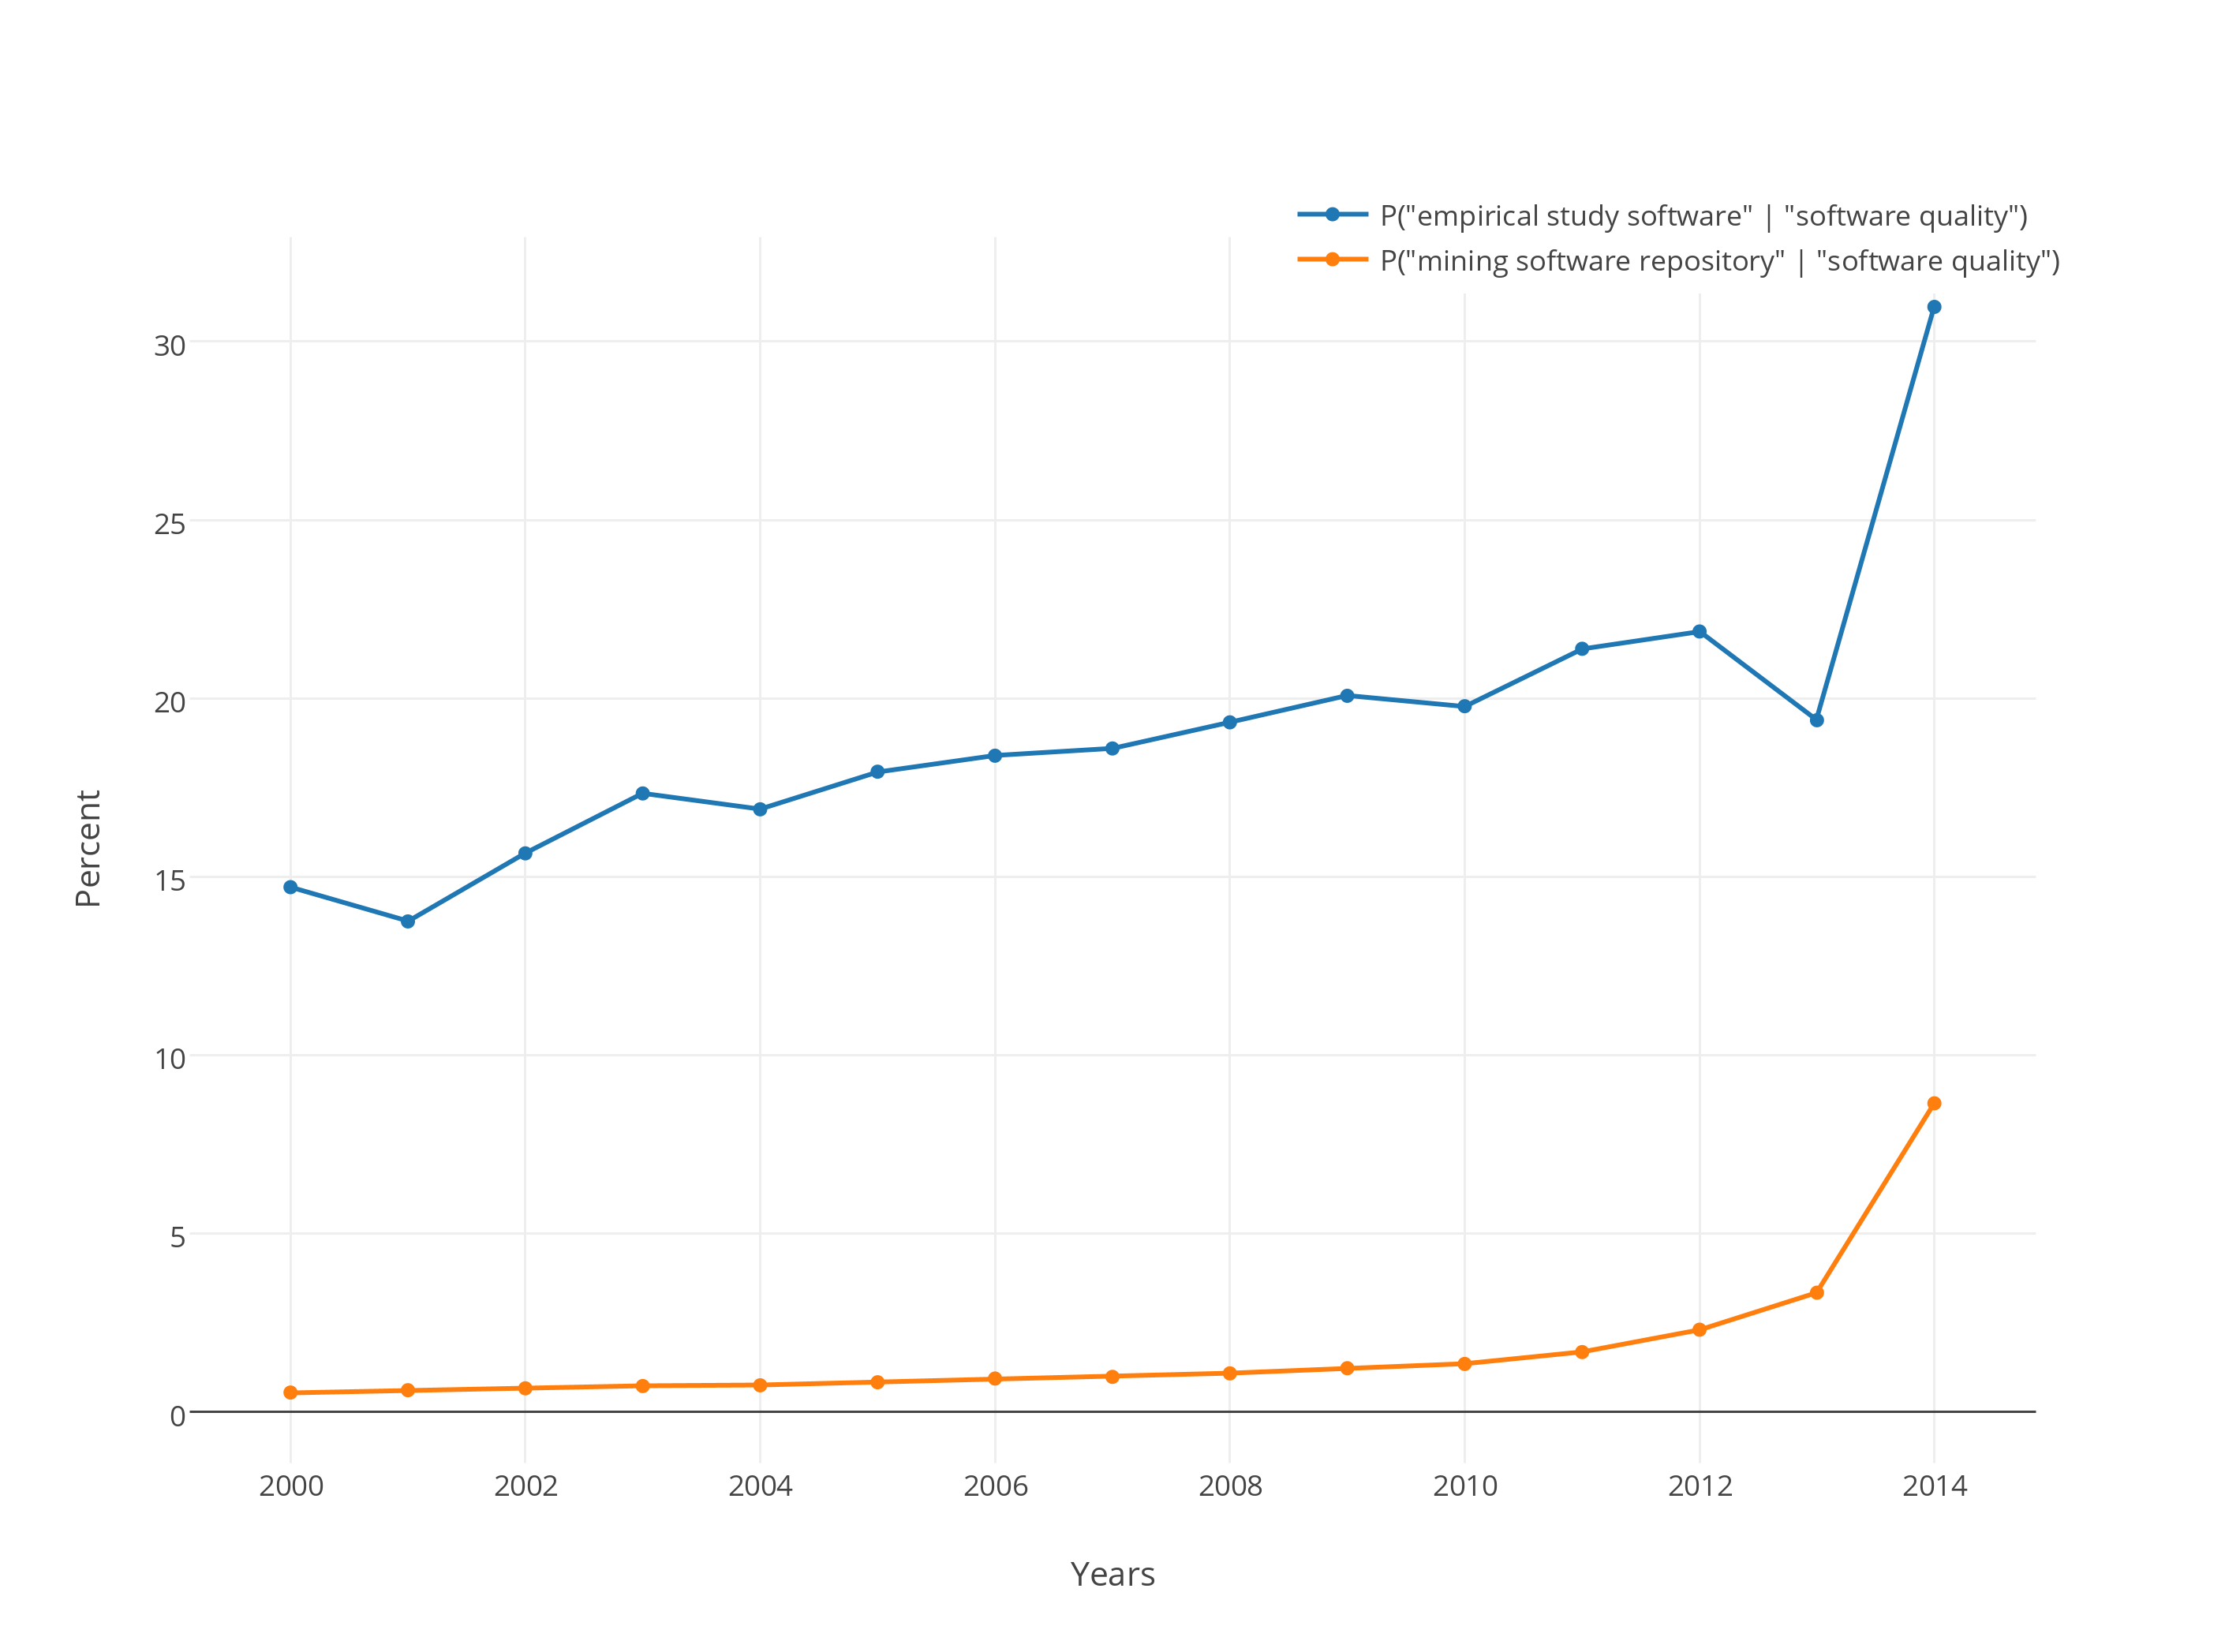
\includegraphics[scale=0.7]{media/scholar.png}
	    \caption{Proportion of papers containing ``Empirical Study'' or ``Mining software repository'' with regards to the paper in Software quality indexed by Google Scholar	\label{fig:scholar}}
	\end{figure}

	\item {\bf Problem 2} : The literature contains numerous paper about tools that improve the overall software quality with static \cite{Dangel2000, burn2003checkstyle,Hovemeyer2007,Moha2010} and dynamic \cite{Nayrolles,Nayrolles2013a,Palma2013} analysis. To the best of our knowledge approaches leveraging other sources to improve quality or efficiency mostly rely on web-search \cite{Brandt2009,Rahman2013,Montandon2013}.

	\item {\bf Problem 3} : There is no approach that support the natural language search and comparison of issues, source code and tasks regardless of the project, repository, revision and issue management system and programming language. Such an approach could dramatically transform software engineering processes. Moreover, the data contained in these repositories lack a taxonomy, as for clone detection \cite{CoryKapser}, to classify the research.
\end{itemize}

\section{Research Challenges\label{sec:challenges}}

\begin{itemize}
	\item {\bf Challenge 1} : Issues \& projects and revision systems are plenty and they all have specific processes and limitations. Mining them all in order to have a representative model is challenging. Despite the parsing aspect, gigabytes of new data are generated every day thus, storing accessing to these data in reasonable time will require innovations in high density nosql databases \cite{Nayrolles2014b} and web servers \cite{Nayrolles2013b,Nayrolles2014c}. Moreover, creating the relationship between both systems is still an open issue as discussed in sections \ref{sec:issue-tracking} and \ref{rel:issue-rela}.

	\item {\bf Challenge 2} : Providing code samples break down to the right level, at the right time in order to solve a problem  or improve the current code in terms of quality, performances or reliability during a programming session will force us to improve current approaches of source code transformation and normalization \cite{Cordy2006a, Cordy2006,Roy2008,Cordy2011}.
	\item {\bf Challenge 3} : 
	\todo{Foramlize a third challenge}
\end{itemize}

\section{Scope of the research \label{sec:scope}}

The area of this research is to improve the processes of software engineering by providing contextual informations, in order to improve the quality, the performance, the reliability of a given code during a programming session. These contextual informations will come from mining issue \& project and revision systems. Hence, we will not define what are the good or bad practices to improve the quality, the performance, the reliability of a given code but rely on the mined data.

\section{Objectives of the thesis\label{sec:objective-thesis}}

This thesis have five main objectives:

\begin{itemize}
	\item To provide a taxonomy of software issues to classify the research.
	\item To propose approaches to aggregate as many issues and revisions systems as possible.
	\item To propose approaches to reproduce field crashes in lab environment using the issue content.
	\item To propose approaches to create a NLP search engine for issues, tasks, commits, patches, fixes.
	\item To create a comprehensive API to access our data.
	\item To propose a context-aware IDE that will improve day-to-day programming session with concise and appropriate code samples.
\end{itemize}

\section{Proposed Solution \label{sec:solution}}

Figure \ref{fig:proposal} depicts our proposed solution for fulfilling the objectives we presented in section \ref{sec:objective-thesis}. 
First of all, a end-user (team member) will report an issue (open a task) in one the organization issues \& project management system. This can be done in $Sourceforge$, $Bugzilla$, $JIRA$ or $Github$ which are the system we want to support first as described in section \ref{sec:bug-provider}.
Issues (tasks) are  mapped with their fixes (implementations) inside {\tt BUMPER} (BUg MetarePository for dEvelopers and Researchers). The source code is fetched from the supported version system: $Git$, $Svn$, $Mercurial$ presented in section \ref{sec:version-control}.  
{\tt BUMPER} is a meta-repository that make issues, tasks and related source code searchable using natural language  (in opposition to structured query language). 
When an issue is reported, {\tt JCHARMING} (Java CrasH Automatic Reproduction by directed Model checkING) will fetch the content of the issue and try to create a scenario to reproduce the on-field crash. In case of success, the developer assigned to this issue will be notified and the scenario stored in {\tt BUMPER}. 
The developer assigned to the task or the issue will modify the code and, in real time, very much like intellisense or auto-completion in modern IDE, {\tt RESEMBLE} (REcommendation System based on cochangE Mining at Block LEvel) will propose improvements or follow up on the developer's code using the decades of history of {\tt BUMPER}. Once s/he is done, s/he submit a commit, patch or diff to the version system. 
However, before s/he allowed to do so, {\tt BIANCA} (Bug Insertion ANticipation by Clone Analysis at commit time) will kicks in and query {\tt BUMPER} looking for similar modifications in other projects and even other programming languages that led to the insertion of a defect in order to warn the user about potential hazardous code.


\begin{figure}[h!]
	\centering
	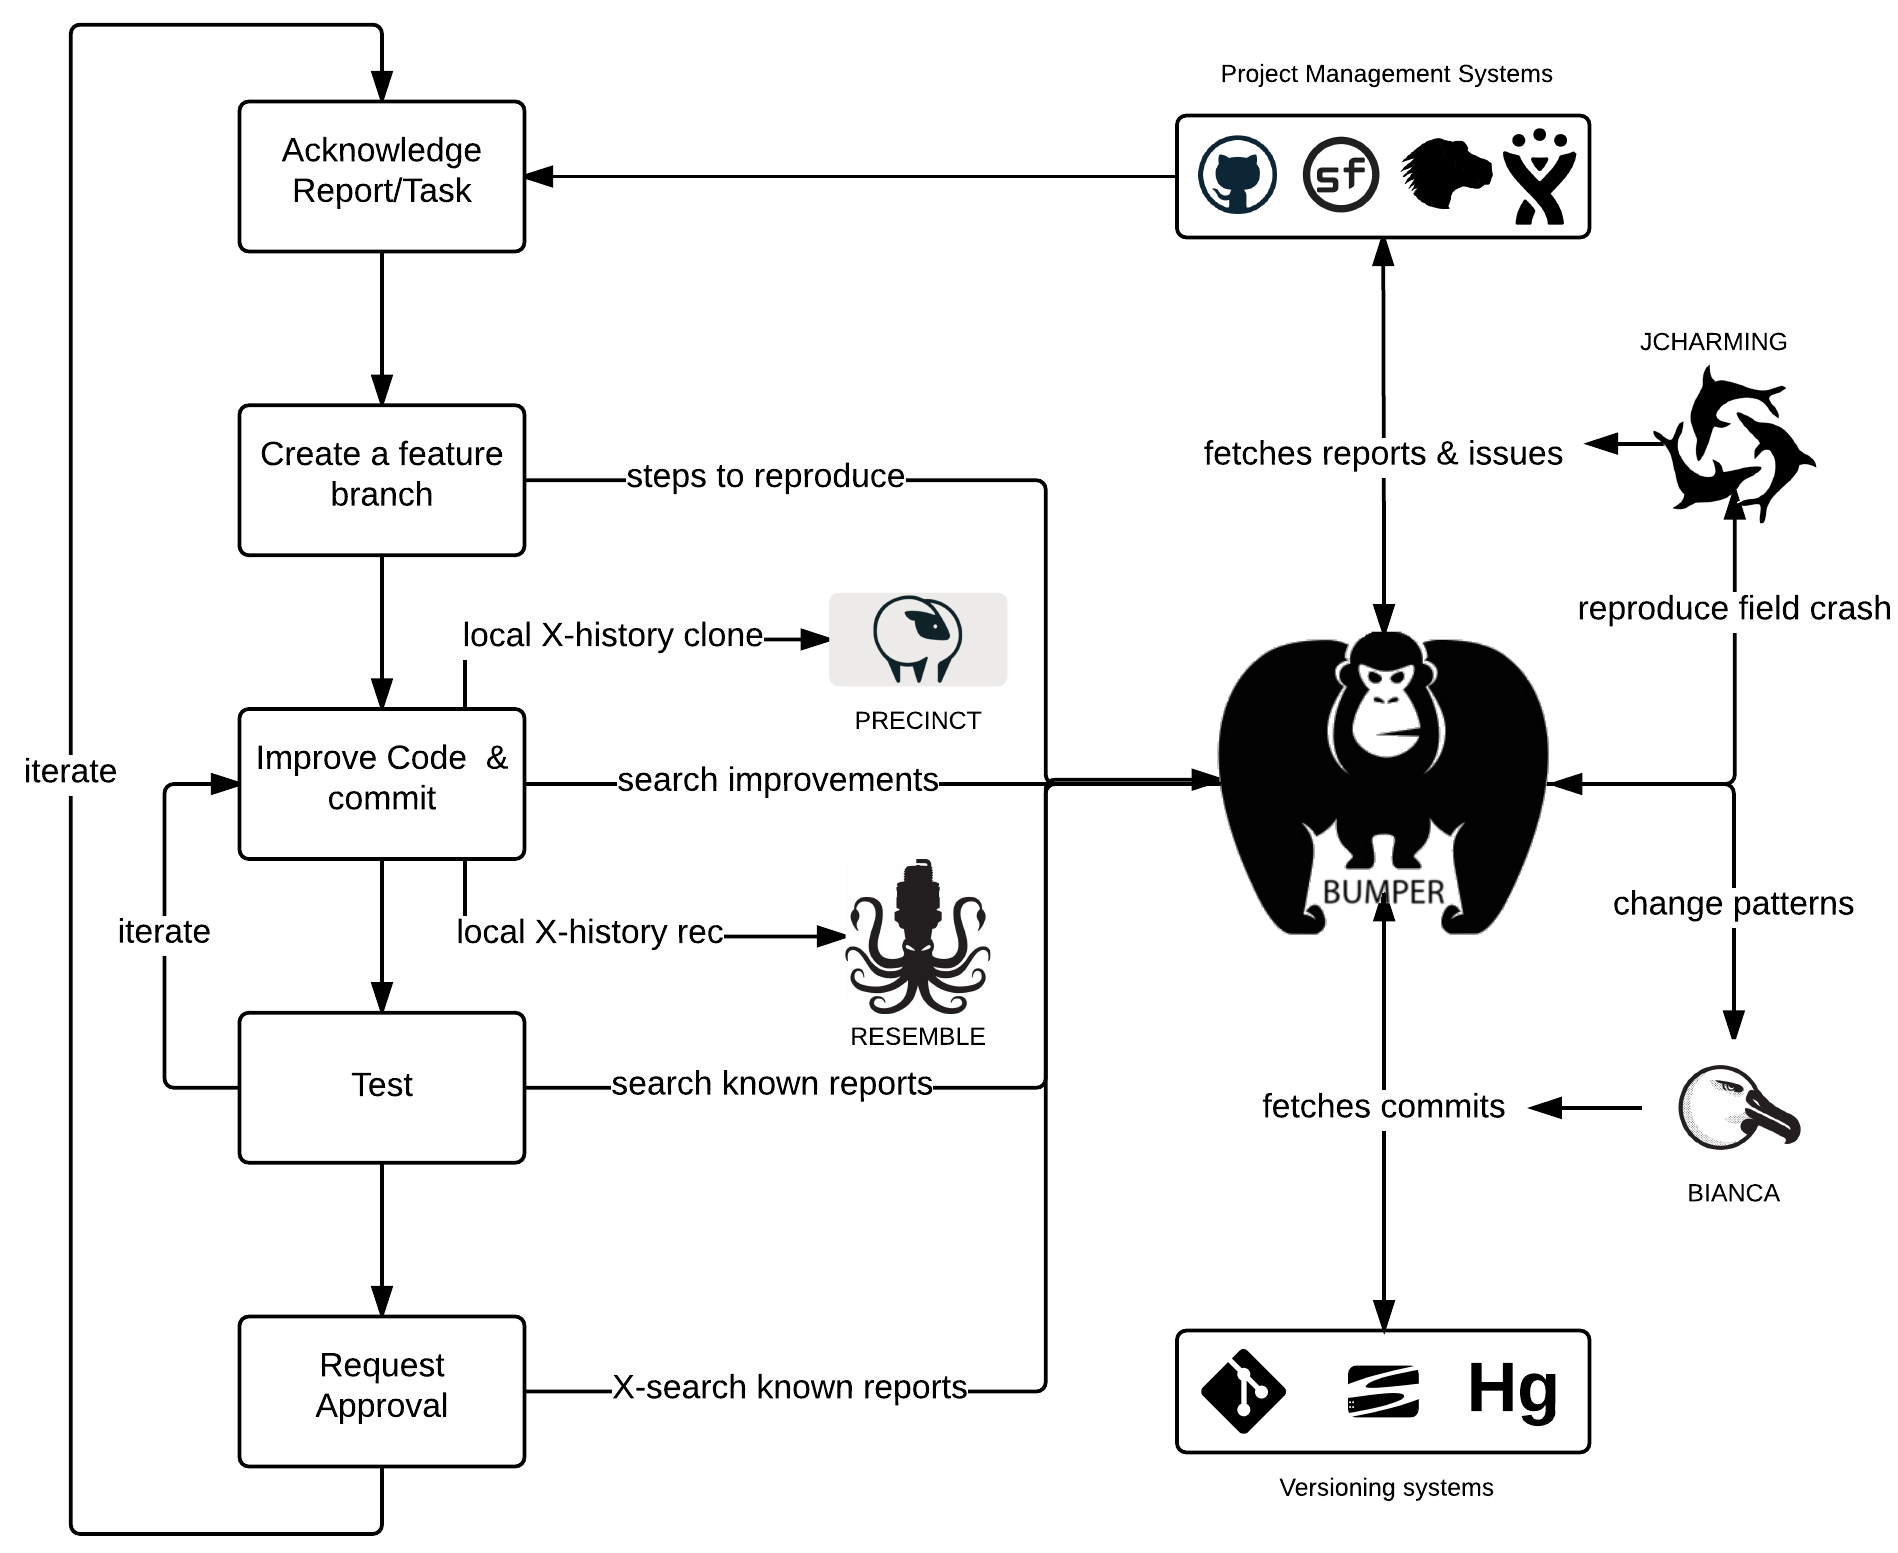
\includegraphics[scale=0.9]{media/proposal.png}
	\caption{Proposed Architecture}
	\label{fig:proposal}
\end{figure}

The bug taxonomy required to build {\tt BUMPER}, {\tt BUMPER} itself, {\tt JCHARMING}, {\tt RESSEMBLE} and {\tt BIANCA} are presented in sections \ref{sec:taxo}, \ref{sec:BUMPER}, \ref{sec:JCHARMING}, \ref{sec:RESEMBLE} and \ref{sec:BIANCA}, respectively. In addition, we list parts that have been published in peer-reviewed conferences in section \ref{sec:current-state} and our publication plan in \ref{sec:publication-plan}.

As a motivating example, we draft the following scenario. Table \ref{tab:bumper-hypo} presents hypothetical data stored in {\tt BUMPER} in terms of sequence \#id, sequence of code blocks, a flag to known if a said sequence introduced an issue in a given system and step to reproduce the issue if any.

\begin{table}[h!]
\centering
\begin{tabular}{c|c|c|c|c}
Seq \#ID & Language \#ID & Blocks & Root of Issue & Steps to reproduce \\ \hline \hline
1        & 1             & A-A-B-C-A-A   & Yes  & E-F-G         \\
2        & 1             & A-A-B-C       & No   & -         \\
3        & 2             & D-E-A-C       & No &  - \\ \hline \hline
\end{tabular}
\caption{Hypothetical {\tt BUMPER} data}
\label{tab:bumper-hypo}
\end{table}

During a programming session, let's assume that a developer have blocks $A-B-C$, then {\tt RESEMBLE} will recommends to transform the current code to $A-A-B-C$ as it seams to be the right thing to do. 
If the developer follows {\tt RESEMBLE} recommendation and then adds another two $A$s and commit his/her changes.
The sequence is now $A-A-B-C-A-A$ and {\tt BIANCA} will raise a warning saying that this sequence is known to be the root of an issue and invite the developer to execute the steps $E-F-G$ -- that were produced by {\tt JCHARMING} -- in order to see if s/he did introduce a defect. Moreover, {\tt BIANCA} will take the time to compare $A-A-B-C-A-A$ and $D-E-A-C$ using our normalization algorithms even if they are not in the same programming language. 
Finally, when a new issue is submitted, {\tt BUMPER} indexes it and {\tt JCHARMING} tries to reproduce it and update the step to reproduce part of {\tt BUMPER}.

We can envision the potential of such a system and the its complexity knowing that it would contain millions of issues, hundreds of thousands projects, dozens of programming languages and will help developers leveraging the knowledge of other developers.

In the next chapter, we discuss the details of the different approaches composing our ecosystem.
